% !TeX root = document.tex
% !TeX encoding = UTF-8 Unicode

\chapter{Conexão}%
\label{chapter:connection}

Os softwares \textbf{Lachesis} e \textbf{moirai} se comunicam através de um
protocolo de rede, mais especificamente o \textit{HTTP} (\textit{HyperText
Transfer Protocol}). Isso possibilita tê-los instalados em diferentes computares
conectados em rede. A configuração para que ambos se comuniquem é simples, sendo
necessário informar apenas o \textit{IP} e a porta onde o \textbf{moirai} está
escutando, esperando por conexões.

Para determinar o \textit{IP} de uma máquina pode-se usar o comando
\mintinline{bash}{ifconfig} no \textit{Linux} ou \textit{macOS} e
\mintinline{bash}{ipconfig} no \textit{Windows}. Caso o computador esteja ligado
a mais de uma rede, como \textit{WiFi} e \textit{Ethernet} (rede cabeada),
deve-se prestar atenção a qual endereço pertence a qual rede físisca. Os
endereços especiais \textit{localhost} e \textit{127.0.0.1} apontam para a
própria máquina, assim, quando usado no \textbf{Lachesis}, ele tentará encontrar
o \textbf{moirai} na mesma máquina em que ele se encontra instalado.

É necessário especificar a porta de conexão, mas essa será sempre \textit{5000},
a não ser que algum \textit{proxy} ou redirecionamento de porta seja empregado.
Para especificar a porta basta adicionar \textit{:5000} ao final do \textit{IP}.
Por exemplo: \textit{localhost:5000} e \textit{192.168.11.1:5000}.

Pode-se ver na Figura~\ref{fig:connect} o módulo de conexão do
\textbf{Lachesis}. Para se conectar a um servidor \textbf{moirai} basta digitar
o endereço de \textit{IP} com a porta e a senha que foi configurada.

\begin{figure}[ht!]
    \centering
    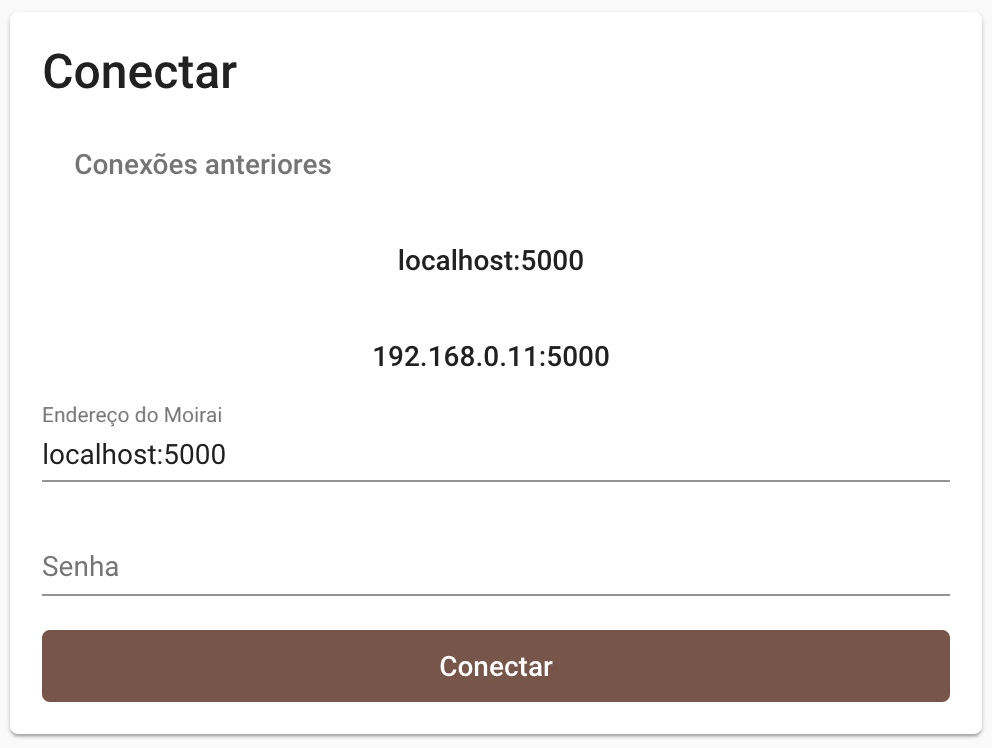
\includegraphics[width=0.9\textwidth]{imgs/connect}
    \caption[Módulo de conexão]{Módulo de conexão}%
    \label{fig:connect}
\end{figure}

Por padrão o endereço \textit{localhost:5000} já vem preenchido. Caso outras
conexões já tenham sido realizadas os endereços serão listados em
\textit{Conexões anteriores}. Basta clicar em um endereço para que ele seja
preenchido no campo correto.

Ao clicar em Conectar algum erro pode ocorrer. Falha de conexão normalmente é
causado por endereço incorreto ou erro na rede. Verifique que o endereço está
certo e que seu computador está de fato na mesma rede que o computador contendo
o \textbf{moirai}. Certifique-se também que o \textbf{moirai} está em execução.
Caso o erro se refira a versão do \textbf{moirai}, esse deve ser atualizado.
Para isso basta executar o comando \mintinline{bash}{pip3 install --upgrade
moirai} em um terminal na máquina onde o \textbf{moirai} se encontra instalado.
Não se esqueça de reiniciar o aplicativo após a atualização.

Uma vez autenticado o módulo de conexão se altera, bem como a barra leteral,
como pode ser visto na Figura~\ref{fig:connection-screen}. A barra lateral exibe
os módulos existentes na plataforma, enquanto o módulo de conexão mostra as
opções de desconectar, alterar senha e salvar/restaurar.

\begin{figure}[ht!]
    \centering
    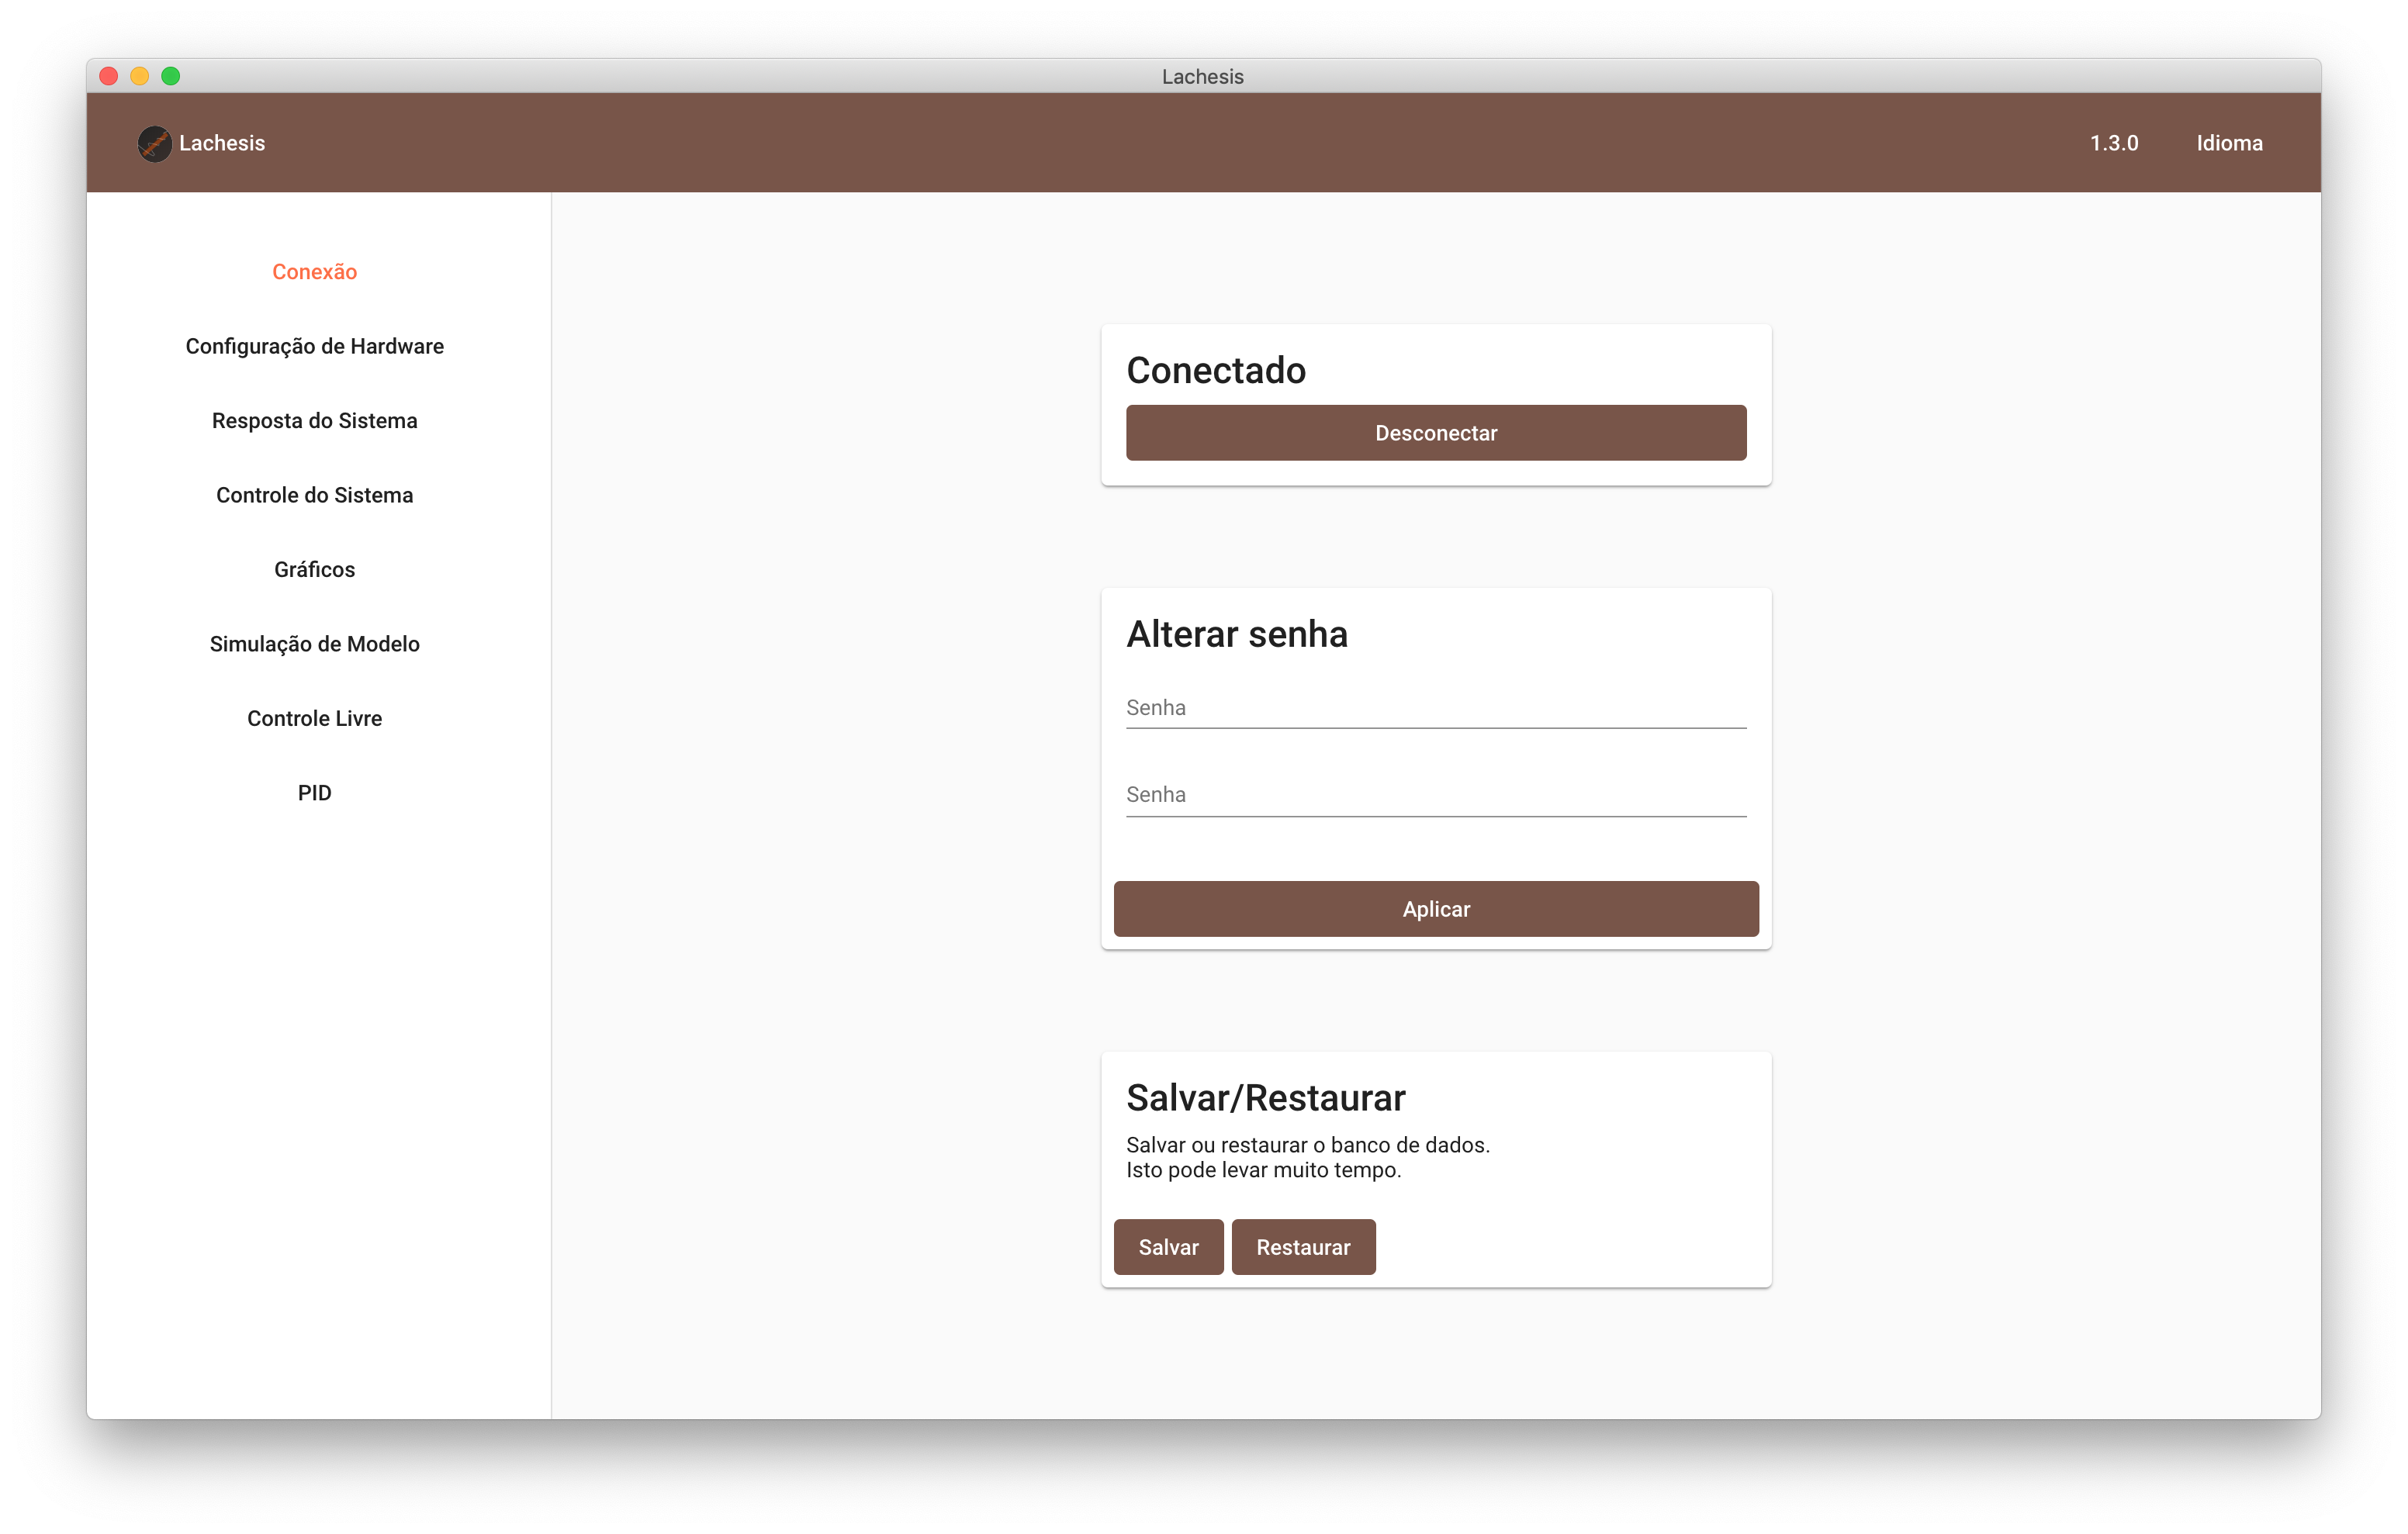
\includegraphics[width=0.9\textwidth]{imgs/connection-screen}
    \caption[Módulo de conexão após autenticação]{Módulo de conexão após autenticação}%
    \label{fig:connection-screen}
\end{figure}

Ao clicar em desconectar o aplicativo volta ao estado inicial, não exibindo os
módulos na lateral e pedindo pelo \textit{IP} e senha.

Para alterar a senha do \textbf{moirai} basta digitar a nova senha duas vezes,
nas duas caixas próprias, e clicar em Aplicar.

As opções Salvar e Restaurar fazem \textit{backup} e restauração de todo o banco
de dados do \textbf{moirai}. Deve-se atentar ao fato que a restauração apaga o
banco atual antes de importar os novos dados, resultando em perda de dados que
não tenham sido salvos em \textit{backup}.

Como o \textit{backup} salva o banco de dados inteiro, os testes realizados
também são salvos. Essa opção pode então ser utilizada para remover dados do
banco, acelerando o aplicativo, sem perder dados. Também pode ser utilizada para
migrar o \textbf{moirai} de uma máquina pra outra.
